
\chapter{Implementation}
\label{chap:implementation}

In this chapter are described implementation details of the project.
Sections in this chapters explains individual problems and their solutions.
The text accompanies actual source code snippets and diagrams for better explanation.


Initially, the project was named as \emph{Malsys} which stands for \emph{Mark's \lsystems} and this name preserved till now.


\section{Solution structure}

The solution is divided into 6 projects: the \lsystem processing library (Malsys), the web user interface (Malsys.Web), the abstract syntax tree (Malsys.Ast), the syntax parser (Malsys.Parsing), the common functionality (Malsys.Common) and the project with tests (Malsys.Tests).

The main reason why the solution do not contain lower amount of projects is because the syntax parser is written in the F\# which is language from .NET family as well as C\# but it is not possible to compile the F\# and C\# into single DLL.
The abstract syntax tree (AST) is separated from the parser because the AST will be compiled by the compilers written in the C\# and it is desirable to have the AST data structures written in the C\#.
It is also more comfortable to design the AST classes in the C\# because the F\# is functional language and the syntax of classes definition is quite complex.
The common functionality is separated into single project because it will be needed in all projects and the solution can not have circular dependencies of projects.
The Web project is separated from main project intentionally to allow usage of the \lsystem processing library independently.
And finally the test project is separated to be possible to test all projects independently.
The dependencies of projects in solution are shown in the \autoref{fig:solutionDependencies}.
The \emph{Malsys.Tests} project has dependencies to all other projects.

\begin{figure}[h]
	\centering
	\begin{tikzpicture}[->,>=latex,shorten >=2pt]
		\node (c) [block] {Malsys.Common};
		\node (m) [block, below=of c] {Malsys};
		\node (a) [block, right=of m] {Malsys.Ast};
		\node (p) [blockx, right=of a] {Malsys.Parsing};
		\node (w) [block, left=of m] {Malsys.Web};
		\node (t) [block, below=2cm of m, xshift=2cm] {Malsys.Tests};
		\node (cSharp) [block, minimum width=1em, minimum height=1em, above=1cm of p] {C\#};
		\node (fSharp) [blockx, minimum width=1em, minimum height=1em, right=0.5cm of cSharp] {F\#};
		
		\draw (a) -- (c);
		
		\draw (p) to[bend right=10] (c);
		\draw (p) -- (a);
		
		\draw (m) -- (c);
		\draw (m) to[bend right=30] (p);
		\draw (m) -- (a);
		
		\draw (w) to[bend left=20] (c);
		\draw (w) -- (m);
		\draw (w) to[bend right=30] (a);
		
		\draw [shorten >=3.4cm] (t) -- (c);
		\draw [shorten >=1.2cm] (t) -- (a);
		\draw [shorten >=2cm] (t) -- (w.south);
		\draw [shorten >=1.2cm] (t) -- (m);
		\draw [shorten >=2cm] (t) -- (p.south);
	\end{tikzpicture}
	\caption{The dependencies of projects in the solution}
	\label{fig:solutionDependencies}
\end{figure}


\section{Input parsing}
\label{sec:parsingImplementaion}

Input parsing is in the \emph{Malsys.parsing} project and it have two phases: lexing and parsing.
The lexing phase uses the lexer to convert the input source code to a stream of \emph{tokens} (basic blocks of input).
The lexer is generated by the \emph{FsLex} tool [\ref{sec:FSharpPowerPack}].
Rules for the \emph{FsLex} are written using regular expressions and the F\# code.
\autoref{code:fsl} shows an example of the lexer definition of the \emph{FsLex} tool.
Full definition is in the file \emph{Lexer.fsl} in the \emph{Malsys.parsing} project.

\begin{Fsharp}[label=code:fsl,caption={Example of the definition file for the \emph{FsLex} tool}]
let whitespace = [' ' '\t']
let digit = '\Nd'  // unicode group for digits
// uppercase, lowercase, titlecase, modifier, other, number (letter)
let letter = '\Lu' | '\Ll' | '\Lt' | '\Lm' | '\Lo' | '\Nl'
// punctuation (connector), nonspacing, spacing, other (format)
let specialChar = '\Pc' | '\Mn' | '\Mc' | '\Cf'
let idFirstChar = letter | '_'
let idChar = letter | specialChar | digit | ['\'']
let id = idFirstChar idChar*

rule tokenize args = parse
    | whitespace { tokenize args lexbuf }  // ignore whitespaces
    | id { match keywords.TryFind(lexeme lexbuf) with
        | Some(token) -> token  // keyword
        | None -> ID(lexeme lexbuf) }  // identifier
    | digit+ { parseInt args lexbuf ConstantFormat.Float }
    ...
\end{Fsharp}

The next phase is called parsing.
The parser is generated by the \emph{FsYacc} tool [\ref{sec:FSharpPowerPack}] from a definition file (\emph{Parser.fsy} in the \emph{Malsys.parsing} project).
The parser is written to parse the input to the abstract syntax tree (defined in \emph{Malsys.ast}).
All data structures in the AST are immutable\footnote{Immutable data structures can not be changed after its creation.} which helps to make the project more robust.
It is impossible to change a value of some AST node by mistake but immutable data structures will not allow this.
\autoref{code:fsl} shows an example of the parser definition.

Both, the \emph{FsLex} and the \emph{FsYacc} tools are run automatically on the build of the project in the Visual studio.

\begin{FsharpBreak}[label=code:fsy,caption={Example of definition file for \emph{FsYacc}}]
// constant definition
ConstDef:
    | LET Id EQUALS Expression SEMI
      { new ConstantDefinition($2, $4, getPos parseState) }
 // function definition     
FunDef:
    | FUN Id OptParamsParens FunBody
      { new FunctionDefinition($2, $3, $4, getPos parseState) }
FunBody:
    | LBRACE FunStatementsList RBRACE
      { new ImmutableListPos<IFunctionStatement>(
      		$2, getPos parseState) }
FunStatementsList:
    |
      { new ResizeArray<IFunctionStatement>() }
    | FunStatementsList FunStatement  { $1.Add($2); $1 }
FunStatement:
    | ConstDef
      { $1 :> IFunctionStatement }
    | RETURN Expression SEMI
      { $2 :> IFunctionStatement }
// identifier
Id:
    | ID
      { new Identifier($1, getPos parseState) }
\end{FsharpBreak}


\section{Compilation and evaluation}

The compilation of the abstract syntax tree is done by a set of compilers defined in the \emph{Compilers} namespace in the \emph{Malsys} project.
There are defined specialized compilers for each part of the AST.
The compilers uses each other to compile the AST.
For example, the \emph{Input compiler} uses the \emph{\lsystem compiler} which uses the \emph{Constant definition compiler}, etc.
\autoref{fig:compilers} shows hierarchy of the compilers.
To keep the figure clear, arrows to the \emph{Expression compiler} was shortened (every compiler uses the \emph{Expression compiler}).

\begin{figure}[h]
	\centering
	\begin{tikzpicture}[->,>=latex,shorten >=2pt]
		\node (in) [block] {Input comp.};
		\node (fd) [block, below=of in] {Function def. comp.};
		\node (ls) [block, left=of fd] {Lsystem comp.};
		\node (cd) [block, right=of fd] {Constant def. comp.};
		\node (ps) [block, left=of in] {Process stat. comp.};
		\node (pa) [block, below=of fd] {Parameters comp.};
		\node (rr) [block, below=of pa] {Rewrite rule comp.};
		\node (sy) [block, below=2cm of ls] {Symbols comp.};
		\node (ex) [block, below right=3cm of fd] {Expression comp.};
		
		
		\draw (in) -- (cd);
		\draw (in) -- (fd);
		\draw (in) -- (ls);
		\draw (in) -- (ps);
		
		\draw (fd) -- (cd);
		\draw (fd) -- (pa);		
		
		\draw (ls) to [bend left=21] (cd);
		\draw (ls) -- (fd);
		\draw (ls) -- (pa);
		\draw (ls) to [bend right=10] (rr);
		\draw (ls) -- (sy);
		
		\draw (ps) -- (ls);
		
		\draw (rr) to [bend right=10] (cd);
				
		\draw (cd) -- (ex);
		\draw (rr) -- (ex);
		\draw [shorten <=1cm] (pa) -- (ex);
		\draw [shorten <=3cm] (fd) -- (ex);
		\draw [shorten <=5.5cm] (sy) -- (ex);
		\draw [shorten <=6.5cm] (ls) -- (ex);
		\draw [shorten <=5cm] (in) -- (ex);
		\draw [shorten <=8.5cm] (ps.south) -- (ex);
	\end{tikzpicture}
	\caption{Hierarchy of the compilers}
	\label{fig:compilers}
\end{figure}


The compilers are not bound to each other statically.
All compilers implements some general interface and they requires other compilers through that interfaces (\autoref{code:compIfaces}).
Each compiler takes all dependent compilers as parameters of the constructor.

\begin{Csharp}[label=code:compIfaces,caption={General interface for the compilers, interface for the constant definition compiler and its implementation}]
// general interface for simplifying definition of compilers interfaces
public interface ICompiler<TSource, TResult> {
	TResult Compile(TSource obj, IMessageLogger logger);
}

// constant definition compiler compiles Ast.ConstantDefinition to ConstantDefinition
public interface IConstantDefinitionCompiler
	: ICompiler<Ast.ConstantDefinition, ConstantDefinition> {}

// concrete implementation of constant definition compiler interface	
public class ConstantDefCompiler : IConstantDefinitionCompiler {
		// constructor
		public ConstantDefCompiler(@IExpressionCompiler expressionCompiler@) { ... }
		// compile method
		public ConstantDefinition Compile(Ast.ConstantDefinition constDefAst,
			IMessageLogger logger) { ... }
}
\end{Csharp}
\nomenclature{IoC}{inversion of control}

An inversion of control (IoC) container is used to instantiate all compilers [\ref{sec:autofac}].
All types of compilers are registered to the IoC container.
Then it is possible to resolve instances of compilers and all theirs dependencies are resolved by the IoC container.
This approach also brings great simplicity and extensibility to the solution.
\autoref{code:compCont} shows the implementation of the compilers container and its possible usage.

\begin{Csharp}[label=code:compCont,caption={General interface for compilers and interface for the expression compiler}]
public class CompilersContainer : ICompilersContainer {
	protected IContainer container;  // the IoC container	

	public CompilersContainer() {
		var builder = new ContainerBuilder();
		builder.@RegisterType<InputCompiler>().As<IInputCompiler>()@.SingleInstance();
		...  // registration of all other compilers
		container = builder.Build();
	}

	public T Resolve<T>() {
		return container.Resolve<T>();
	}
}

// possible usage
var inputContainer = new CompilersContainer().@Resolve<IInputCompiler>()@;
\end{Csharp}

The result of compilation is a semantic tree (ST).
The semantic tree is as well as the AST immutable.

All compilation errors are logged with the \emph{IMessageLogger} class.
No exceptions are thrown which helps the performance and error recovery (compiling can continue even after non fatal errors). 


\subsubsection*{Evaluation}

Evaluation of the semantic tree is implemented in the same way as the compilation.
There is set of evaluators and an IoC container that links them together.



\section{Components members}
\label{sec:compImplementaion}

A component is the .NET class.
All components must implement the \emph{IComponent} interface (\autoref{code:IComponent}) and they must have a parameter-less constructor.

\begin{Csharp}[label=code:IComponent,caption={Interface of the \emph{ProcessManager} class}]
public interface IComponent {
	IMessageLogger Logger { set; }
	void Initialize(ProcessContext context);
	void Cleanup();
}
\end{Csharp}

According to \autoref{sec:components}, any component can have: settable properties, settable symbol properties, gettable properties, connection properties, callable functions and interpretation methods.
All listed members are marked with special attributes to be possible to distinguish from other class properties and methods.
The access name of all members is the same as their real name, however, the \emph{AccessName} attribute can be used to change it.


\subsubsection{Component lifetime}
\label{sec:componentLifetime}

The \emph{IComponent} have two basic methods: the \emph{Initialize} and the \emph{Cleanup}.
Following list shows the order of individual operations during creation of the component graph.

\begin{itemize*}
	\item instantiation (using required parameter-less constructor),
	\item set of \emph{Logger} property
	\item for each processed \lsystem:
	\begin{itemize*}
		\item reset (cleanup) with the \emph{Cleanup} method, it should be used for setting the component to a default state
		\item connecting of other components (setting the connection properties)
		\item setting of the settable (symbol) properties
		\item initialization with the \emph{Initialize} method
		\item processing of the \lsystem
	\end{itemize*}
	\item cleanup with \emph{Cleanup} method.
\end{itemize*}



\subsubsection{Settable properties}

The settable properties (and the settable symbol properties) are actual properties of the component class marked with the \emph{UserSettable} (\emph{UserSettableSybols}) attribute.
The properties must have a public setter (a getter is not required).
The settable properties must have their type assignable to the \emph{IValue} which covers both base types, the numbers (\emph{Constant} type) and the arrays (\emph{ValuesArray} type).
The settable symbol properties must have \emph{ImmutableList<Symbol<IValue>{}>} type.

By default, all settable (symbol) properties are "optional" which means that their value may not be set.
By setting the \emph{IsMandatory} property of the \emph{UserSettable} (\emph{UserSettableSybols}) attribute to true, the property is marked as mandatory and an error will be thrown if no value is set to it.

The setter of the settable (symbol) properties can throw the \emph{InvalidUserValueException} if the supplied value is invalid.
The text of the exception will be shown as an error to the user.



\subsubsection{Gettable properties}

Similarly as the settable properties, the gettable properties are actual properties of the component class marked with the \emph{UserGettable} attribute.
The properties must have a public getter (a setter is not required) and their type must assignable to the \emph{IValue} type.

By default, values of the gettable properties can be get after the initialization of the component.
In that time all the statements from processed \lsystem are already evaluated, thus the value of the gettable properties can not be used in them.
However, it is possible to set the \emph{IsGettableBeforeInitialiation} property of the \emph{UserGettable} attribute to allow getting oft the property value before the initialization and to use the value in the \lsystem statements.


\subsubsection{Connection properties}

The connection properties are for connecting other components.
They are actual properties of the component class marked with the \emph{UserConnectable} attribute.
Properties must have a public setter (a getter is not required) and their type must be assignable to the \emph{IComponent} type.

Connection of some component to the connection properties is, by default, mandatory but it is possible to set the \emph{IsOptional} property of the \emph{UserConnectable} attribute to allow leaving the property unconnected (\emph{null}).
By default, only one component can be assigned (connected) to each connection property but this can be changed by the \emph{AllowMultiple} property of the \emph{UserConnectable} attribute.

The setter of connection property can throw the \emph{InvalidConnectedComponentException} if supplied value of a component is invalid.
The text of the exception will be shown as an error to the user.


\subsubsection{Callable functions}

Callable functions serves to allow calling of component methods in \lsystem code (in statements, rewrite rules etc.).
Callable functions are method of the component class marked with the \emph{UserCallableFunction} attribute.
The underlying method must have two parameters parameter of types \emph{IValue[]} and \emph{IExpressionEvaluatorContext}.
The return type of the method must be assignable to the \emph{IValue} type.

Similarly as gettable properties callable functions can be by default called after the initialization of the component but it is possible to set the \emph{IsCallableBeforeInitialiation} property of the \emph{UserCallableFunction} attribute to allow calling the function before the initialization.


\subsubsection{Interpretation methods}

The interpretation methods are specialized methods used for interpretation of \lsystem symbols.
The interpretation methods must be marked with the \emph{SymbolInterpretation} attribute, they must have a parameter of type \emph{ArgsStorage} and \emph{void} return type.


\subsection{Documentation of members}
\label{sec:componentDoc}

\nomenclature{DLL}{dynamic-link library}
To simplify the documentation of a component and their members the standard \emph{XmlDoc} with custom elements is is used for documentation.
The documentation is loaded automatically if the XML file with the documentation is included with the DLL where the component is located.

Standard \emph{summary} tag is used to document the component.
The \emph{user readable name} for the component can be written in the \emph{name} tag and for the name of \emph{group} to which the component belongs is the tag called \emph{group}.
Example of the documentation of a component is in \autoref{code:docExample}.

\begin{Csharp}[label=code:docExample,caption={Example of usage the XmlDoc for documentation of a component}]
/// <summary>
///	Provides symbol property called Axiom which serve as
/// initial string of symbols of L-system.
/// </summary>
/// <name>Axiom provider</name>
/// <group>Common</group>
public class AxiomProvider : SymbolProvider {
	...
}
\end{Csharp}



\subsubsection{Settable (symbol) properties}

Basic documentation is of a settable property is loaded from the \emph{summary} tag.
Expected value description can be put into the \emph{expected} tag and for the default value of a settable property is the \emph{default} tag.

For settable symbol properties is loaded only the \emph{summary} tag


\subsubsection{Gettable and connection properties}

Documentation for gettable and connection properties is loaded from standard \emph{summary} tag.


\subsubsection{Callable functions and interpretation methods}

In addition to standard \emph{summary} tag for general documentation, callable functions (and interpretation methods) can be documented with the \emph{parameters} tag where on each line should be documentation for each parameter. 


\subsection{Example}

The example of implementation and the documentation of a component is in appendix \ref{chap:compImpl}.


\section{Input processing}
\label{sec:implInputProcessing}

Component graph creation is the core of the \lsystem processing library.
The class responsible for that is called the \emph{ProcessManager} (\autoref{code:procMan}).

It uses the class \emph{ProcessConfigurationBuilder} for creation and configuration of the component graph.
For resolving component types the \emph{ProcessManager} uses the \emph{IComponentMetadataResolver}.
It works in the similar way as the IoC container but the components do not have any dependencies.
The components are registered by the user directly using the \emph{IComponentMetadataResolver} implementation or with the helper class called \emph{MalsysLoader}.

\begin{Csharp}[label=code:procMan,caption={Interface of the \emph{ProcessManager} class}]
public class ProcessManager {

	public ProcessManager(ICompilersContainer compIoc,
		IEvaluatorsContainer evalIoc, @IComponentMetadataResolver compResolver@) {

	public InputBlockEvaled CompileAndEvaluateInput(string sourceCode,
		string sourcName, IMessageLogger logger) { ... }
		
	public void @ProcessInput@(InputBlockEvaled inBlock, IOutputProvider outProvider,
		IMessageLogger logger, TimeSpan timeout) { ... }
}
\end{Csharp}

The \emph{ProcessManager} does following steps in the method \emph{ProcessInput}.
Notice the similarities with the compoennt lifetime (\autoref{sec:componentLifetime}).

For each process statement in the input do:
\begin{enumerate*}
	\item instantiate all components in the Process configuration (specified by the process statement),
	\item \label{procStep2} save the gettable properties and the callable functions from all components which can be get and called before the initialization,
	\item for each \lsystem (specified by the process statement) do:
	\begin{enumerate*}
		\item reset (clean) all components,
		\item connect all components to the graph (resetting may disconnect them),
		\item evaluate the \lsystem,the  gettable properties and the callable functions from step \ref{procStep2} can be used to evaluate the \lsystem statements,
		\item evaluate additional \lsystem statements from the process statement,
		\item set the settable properties of all components (from evaluated \lsystem statements),
		\item save rest of the gettable properties and the callable functions from all components,
		\item initialize all components,
		\item find the starter component and start it,
	\end{enumerate*}
	\item reset (clean) all components.
\end{enumerate*}


\section{Immutable data structures as scoped storage}
\label{sec:immutableDs}

In many places in the \lsystem processing library there is need for temporary addition of constants to a collection.
As an example can be evaluation of a function.
The parameters of the function are added as constants to the a collection but this addition can overlay already defined constants.
After the evaluation, the collection should be in the same state as before (parameters and local variables must not remain).
This problem can be solved by complex mutable data structures or by defensive copying of the collection which can lead to serious performance issues (there can be hundreds of defined constants).

\emph{Immutable data structures} offers clean solution to this problem.
An immutable data structure is data structure which can not be changed (muted) such as the \emph{string} in the C\#.
They can not be changed, thus there is no need for creation of defensive copies.
If a method passes an immutable collection of defined constants to the function evaluation method the collection can not be changed by it.

But how is possible to add new items to immutable data structures if they can not be changed?
It is not possible because they are immutable but it is possible to create a new copy with added item.
Interestingly enough, addition to an immutable tree has the same asymptotic complexity as insertion to a mutable one.

Each node of the immutable tree is immutable.
If we want to add new node we will find the place in the tree where it should be.
Now we need to connect it to the parent but the parent is immutable so we will create new parent (copying value from old one) but with new connections.
Old children (if any) can be connected without re-creating them.
So we need to re-create only nodes on the path to the root so complexity is logarithmic ($log_2(n)$ new nodes).
Insertion to the immutable tree is illustrated in \autoref{fig:immAdd}.

There is no need for implementation of immutable tree because the F\# contains it as the \emph{FSharpMap<TKey, TValue>} class and the \emph{MapModule} class provides methods for the work with it.

Described system ensures that global variables will be accessible and can be temporarily overlayed by more local definitions.
It is used in may places such as evaluation of the \lsystems (local constants and functions overlays global ones), evaluation of user-defined functions (parameters and local variables)
	and the rewrite rules (parameters of symbols are mapped as local variables).
	

\tikzstyle{tree} = [draw, fill=blue!12, circle, minimum size=9mm]
\tikzstyle{treex} = [draw,thick, fill=red!12, circle, minimum size=9mm]

\begin{figure}[h!]
	\centering
	\subfloat[Original tree]{
	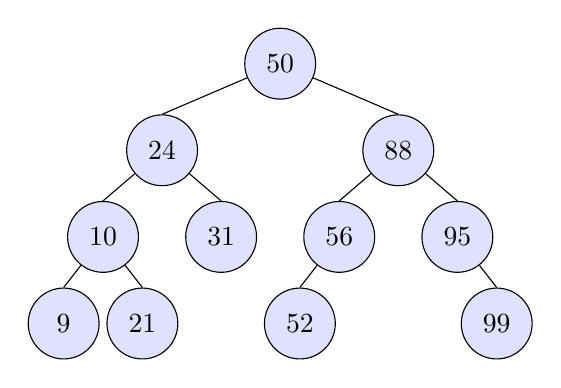
\begin{tikzpicture}[child anchor=north,>=latex,level/.style={sibling distance=30mm/#1},level distance=11mm]
		\node [tree] {50}
			child { node [tree] {24}
				child {node [tree] {10}
					child { node [tree] {9} }
					child { node [tree] {21} }
				}
				child { node  [tree] {31} }
			}
			child { node [tree] {88}
				child { node [tree] {56}
					child { node [tree] {52} }
					child [missing] {}
				}
				child { node [tree] {95}
					child [missing] {}
					child { node [tree] {99} }
				}
			}
			;
	\end{tikzpicture}
	} \hfill
	\subfloat[Tree with inserted node 71]{
	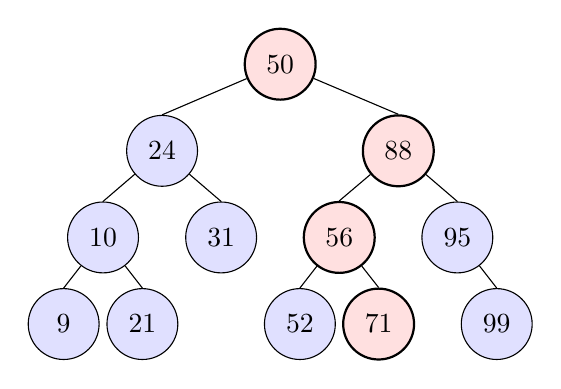
\begin{tikzpicture}[child anchor=north,>=latex,level/.style={sibling distance=30mm/#1},level distance=11mm]
		\node [treex] {50}
			child { node [tree] {24}
				child {node [tree] {10}
					child { node [tree] {9} }
					child { node [tree] {21} }
				}
				child { node  [tree] {31} }
			}
			child { node [treex] {88}
				child { node [treex] {56}
					child { node [tree] {52} }
					child { node [treex] {71} }
				}
				child { node [tree] {95}
					child [missing] {}
					child { node [tree] {99} }
				}
			}
			;
	\end{tikzpicture}
	}
	\caption[Example of the add operation to the immutable tree]{Example of the add operation to the immutable tree, red nodes are newly created}
	\label{fig:immAdd}
\end{figure}


\section{Implemented components}

There are many implemented components in the \lsystem processing library.
In this section is described implementation details of some of them.


\subsection{Symbol rewriter}

The core of the \lsystem processing is the rewriting of \lsystem symbols.
The \emph{SymbolRewriter} component is responsible just for that.
Its implementation supports all \lsystem types described in \autoref{sec:lsysTypes}.

The most complicated of the \emph{SymbolRewriter} component is the context checking (in context rewrite rules, see \autoref{sec:bracketedLsystems}).
The context checking can not be implemented by naive approach which will search the context of symbol one by one because branches must be skipped and they can be very long.
\autoref{lsys:longContext} demonstrates an \lsystem where the naive implementation will not be able to work well.
It uses symbol \texttt{S} to generate random color index as its parameter.
Symbol \texttt{S} is "linked" using the context to every symbol \texttt{X} which is rewritten to new branches with color index from the base symbol \texttt{S}.
This causes that all lines in one iteration have the same color but colors between iterations differs.
First five iterations with the random seed set to 0 are shown in \autoref{fig:longContext}.

\begin{Lsystem}[label=lsys:longContext,caption={\lsystem }]
lsystem LongContext extends Branches {
	set symbols axiom = S(0) X;
	set symbols @contextIgnore = + - F@;
	set iterations = 5;
	set initialAngle = 90;	
	interpret F(c) as DrawForward(32, 2, c * #001100);
	interpret + as TurnLeft(20);
	interpret - as TurnLeft(-20);
	rewrite @{S(c)} X@ to [ + F(c) X ] - F(c) X;
	rewrite S to S(floor(random(0,16)));
}
process all with SvgRenderer;
\end{Lsystem}

\begin{figure}[h]
	\subfloat{\includegraphics[scale=0.9]{LongContext1}} \hfill
	\subfloat{
\includegraphics[scale=0.85]{LongContext2}} \hfill
	\subfloat{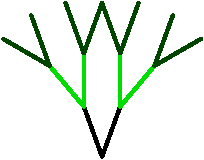
\includegraphics[scale=0.8]{LongContext3}} \hfill
	\subfloat{\includegraphics[scale=0.75]{LongContext4}} \hfill
	\subfloat{\includegraphics[scale=0.7]{LongContext5}}
	\caption{Result of \lsystem in \autoref{lsys:longContext}}
	\label{fig:longContext}
\end{figure}


In the following list are strings of symbols of the first five iterations of the \lsystem in \autoref{lsys:longContext}.
Ignored symbols \texttt{-} and \texttt{F} are omitted.
Every symbol \texttt{X} needs to search for the very first symbol to match the context correctly.
Now you can see why the naive implementation can not be used.

\begin{enumerate*}
	\item S(0) X
	\item S(11) [ X ] X
	\item S(13) [ [ X ] X ] [ X ] X
	\item S(12) [ [ [ X ] X ] [ X ] X ] [ [ X ] X ] [ X ] X 
	\item S(8) [ [ [ [ X ] X ] [ X ] X ] [ [ X ] X ] [ X ] X ] [ [ [ X ] X ] [ X ] X ] [ [ X ] X ] [ X ] X 
\end{enumerate*}

The \emph{SymbolRewriter} component builds a tree from the symbols which allows to skip the branches quickly.
The nodes of the tree at the same level are interlinked to allow search for the left and the right context effectively.
The pointer to the current symbol is updated after each processed symbol.
The tree is dynamically loaded as the right context needs more symbols.
The tree node is represented by the \emph{ContextListNode<T>} class.
The \emph{ContextListBuilder} class helps to build the tree correctly symbol by symbol.

The search tries all possible ways to match the context but number of possible ways is relatively low.
\autoref{fig:contextChecking} shows an example of the context search in the tree built from the fourth iteration of the \lsystem in \autoref{lsys:longContext}.
The red path shows search for the left context \texttt{S} of the symbol \texttt{X} and the green path shows the search for the right context \texttt{[X]} of the symbol \texttt{X}.
The search methods are located in the \emph{ContextChecker} class.

\tikzstyle{arr} = [draw, fill=blue!12, rectangle, minimum height=2em, minimum width=2em]
\tikzstyle{sym} = [draw, fill=red!12, rectangle, minimum height=2em, rounded corners=1mm]
\tikzstyle{arrow} = [draw=gray,<->,dashed,shorten >=2pt,shorten <=2pt]
\tikzstyle{path} = [draw=red,thick,->,shorten >=1pt]
\tikzstyle{path2} = [draw=green,thick,->,shorten >=1pt]

\begin{figure}[h!]
	\centering
	\begin{tikzpicture}[child anchor=north,>=latex,level/.style={sibling distance=33mm/#1}]
		\node [arr,] {root}
			child { node (a) [sym,draw=red, thick] {S(12)} }
			child { node (b) [arr] {[ ]}
				child { node (ba) [arr] {[ ]}
					child { node (baa) [arr] {[ ]}
						child { node (baaa) [sym] {X} }
					}
					child { node (bab) [sym] {X} }
				}
				child { node (bb) [arr] {[ ]}
					child { node (bba) [sym,draw=green, thick] {X} }
				}
				child { node (bc) [sym,draw=red, thick] {X} }
			}
			child { node (c) [arr] {[ ]}
				child { node (ca) [arr] {[ ]}
					child { node (caa) [sym] {X} }
				}
				child { node (cb) [sym] {X} }
			}
			child { node (d) [arr] {[ ]}
				child { node (da) [sym] {X} }
			}
			child { node(e) [sym] {X} }
			;
		\draw [arrow] (a) -- (b);
		\draw [arrow] (b) -- (c);
		\draw [arrow] (c) -- (d);
		\draw [arrow] (d) -- (e);
		
		\draw [arrow] (ba) -- (bb);
		\draw [arrow] (bb) -- (bc);
		
		\draw [arrow,dashed,shorten >=0,shorten <=0] (baa) -- (bab);
		
		\draw [arrow] (ca) -- (cb);
		
		\draw [draw=red,<-,thick,shorten <=2pt] (bc) -- +(0,-2cm);
		\draw [path] (bc) to[bend right=20] (bb);
		\draw [path] (bb) to[bend right=20] (ba);
		\draw [path,dashed] (ba) to[bend right=20] +(-1.2cm,0);
		\draw [path] (ba.north) ++(-0.2,0) to[bend left=20] (b);
		\draw [path] (b) to[bend right=20] (a);
		
		
		\draw [draw=green,<-,thick,shorten <=2pt] (bba) -- +(0,-2cm);
		\draw [path2] (bba) to[bend right=20] (bb);
		\draw [path2, dashed] (bb) to[bend right=20] (bc);
		\draw [path2] (bb) to[bend right=20] (b);
		\draw [path2] (b) to[bend left=20] (c);
		\draw [path2,dashed] (c) to[bend right=20] (ca);
		\draw [path2] (c) to[bend left=20] (d);
		\draw [path2] (d) to[bend right=20] (da);
		
		\node [area,fit=(d) (da),thick,green] {};
	\end{tikzpicture}
	\caption[The context search tree]{The context search tree built from the fourth iteration of the \lsystem in \autoref{lsys:longContext}}
	\label{fig:contextChecking}
\end{figure}

As a context matching method finds matching symbol it also maps its parameters as new constants.
Because the context matching is done by the back-track and the mapped symbols can be invalid, immutable data structures are used for saving the mapped constants.
Because of immutable data structures the roll-back to old values can be done with no cost (see \autoref{sec:immutableDs}).
Described algorithm is not optimal but it is sufficient for the most cases.
Production \lsystem have rarely context longer than one.

The context checking is tested by many unit tests in the \emph{Malsys.Tests} project which ensures correctness of implemented algorithm.


\subsection{Turtle graphics interpreter}

A turtle graphics interpreter is universal interpreter for both 2D and 3D renderers and it is implemented by the class \emph{TurtleInterpreter}.
It interprets \lsystem symbols as a \emph{turtle graphics} in 3D but if 2D renderer is connected it omits the Z coordinate.
This allows to use 3D commands even if 2D rendered is connected which brings many advantages.
For example, the \emph{Roll} (a rotation by the direction axis) by $180^{\circ}$ can be used for the inversion of turning directions in 2D.

The interpreter allows to use three basic rotations: \emph{pitch}, \emph{yaw} and \emph{roll}.
The pitch operation turns "up" around right-hand vector, the yaw turns "left" around up vector axis and the roll operation rolls clock-wise around forward vector axis.
The up, right and forward vectors can be set by the user using the settable properties.
This allows some changes to the coordinate system for example, the forward and right vectors may not right-angled.

The rotation of the turtle is represented as the \emph{Quaternion}.
This has many advantages over "traditional" representation with a rotation matrix.
Quaternions represent a rotation around some axis which is exactly what the basic operations do.
In the contrast to representation by the rotation matrix, the quaternion allows to do pitch, yaw and roll by axes which are relative to current orientation easily.
Also the storage size of the rotation represented by the quaternion is the smallest possible since the quaternion is represented as four numbers.
Composition of two quaternion rotations is equal to multiplying the quaternions.
\autoref{code:yaw} shows a code snippet of the \emph{Yaw} interpretation method of the \emph{TurtleInterpreter}.


\begin{Csharp}[label=code:yaw,caption={Implementation of the \emph{Yaw} method of the \emph{TurtleInterpreter}}]
[SymbolInterpretation(1)]
public void Yaw(ArgsStorage args) {
	double angle = getArgumentAsDouble(args, 0);
	currState.Rotation *= new Quaternion(upVect, angle);
}
\end{Csharp}


The \emph{TurtleInterpreter} can simulate the tropism\footnote{A tropism is a biological phenomenon, indicating growth or turning movement of a biological organism, usually a plant, in response to an environmental stimulus (\url{http://en.wikipedia.org/wiki/Tropism}).}.
This is easily done by quaternions too because the tropism is simulated as a physical force which is applied to the line as you can see in \autoref{code:tropismImpl}~\cite[p.~58]{PL91}.

\begin{Csharp}[label=code:tropismImpl,caption={Implementation of the tropism which is applied after each line}]
private void rotateByTropism(Vector3D moveVector) {
	Vector3D axis = Vector3D.CrossProduct(moveVector, tropismVect);
	double angle = axis.Length * tropismCoef;
	if (angle.EpsilonCompareTo(0) == 0) {
		return;
	}
	axis.Normalize();
	currState.Rotation = new Quaternion(axis, angle) * currState.Rotation;
}
\end{Csharp}


\section{Triangulation of 3D polygons}

Turtle graphics interpretation of the \lsystems can generate polygons which are objects in the space that are defined the points on its.
These objects are regular polygons in 2D nad they are is easy to render even if its shape is complex (crossing edges, etc.).
But in 3D the situation is much more complex.
Lets call the object specified by points on its perimeter \emph{3D polygon} even if it is not 100\% technically correct.
The 3D polygon is specified by the points on its perimeter but they does not say anything about the shape in the middle.

The easiest way how to render general shapes in 3D is to compose them from triangles.
The conversion process from 3D polygon to triangles is called triangulation.
There is more possible triangulations even of basic 3D polygons (see the situation for four points is in \autoref{fig:3dSquare}).

\begin{figure}[h!]
	\hfill
	\subfloat{\includegraphics[width=0.3\linewidth]{3dSquare1}}
	\hfill
	\subfloat{\includegraphics[width=0.3\linewidth]{3dSquare2}}
	\hfill ~
	\caption{Ambiguous triangulation of four points}
	\label{fig:3dSquare}
\end{figure}

Because of the ambiguity in the triangulation there can not exist an ideal triangulation algorithm.
With this in the mind was written the trianguler in the \lsystem processing library.
It is possible to configure triangulation strategies.

The triangulation algorithm works on the \emph{cutting-ear} base.
From each point of the 3D polygon can be created a triangle (called \emph{ear}) by connecting the point to its two neighbors.
Then one ear is picked (by strategy which is given by the user) and \emph{cut off} which means that the triangle is sent to the output.
Remains a polygon with one less point and the cutting is repeated until only 3 points remains.

The only thing which can be affect by user is the order of the cutting but it is quite enough.
This algorithm is implemented in the \emph{Polygon3DTrianguler} class and the triangulation method takes as an argument (besides actual points) \emph{triangulation parameters} which specifies:
	\begin{inparaenum}[{\itshape a})]
		\item the evaluation delegate which is used for evaluation of ears,
		\item the ordering of ears' scores (ascending or descending) which specifies whether minimal or maximal score is the best,
		\item the recount mode which can be set to \emph{never}, \emph{neighbors} or \emph{all}; it specifies what ears are reevaluated after the cutting, and
		\item attached multiplier, after the cutting the evaluation score of neighboring ears are multiplied with it.
	\end{inparaenum}
	
The algorithm also have support for detection of planar polygons because the turtle graphic tends to produce planar polygons in 3D space.
It tries to find a plane where the polygon is planar by finding some plane and counting the coefficient of variation of distance from the plane to all points
	(the ratio of the standard deviation $\sigma$ to the mean $\mu$).
If the coefficient is under the threshold (given by the user) the polygon is projected on found plane and standard Delaunay triangulation algorithm is used for robust triangulation.


The triangulation algorithm is very versatile but to simplify its usage there is defined 5 strategies.

\begin{description*}
	\item[As in input] -- cuts ear one by one from the first to the last point without any sorting
	\item[Minimal angle] -- triangles with minimal angles are triangulated first
	\item[Maximal angle] -- triangles with maximal angles are triangulated first
	\item[Maximal distance] -- triangles with maximal distance from all points are triangulated first
	\item[Maximal distance from non-triangulated] -- triangles with maximal distance from non-triangulated points are triangulated first
\end{description*}

The user can pick one of the strategies that gives the best results to their polygon type.
The choice can be done by setting the \emph{polygonTriangulationStrategy} property of the \emph{ThreeJsSceneRenderer3D} component.
The standard library contains constants which can be used instead of "magic" numbers to keep the code readable (appendix \ref{sec:stdLibThreeJs}).
\autoref{fig:triangulationSpiral} shows complex 3D polygon triangulated with three different strategies.

\begin{figure}[h!]
	\subfloat[Maximal angle]{\includegraphics[width=0.3\linewidth]{SpiralErr1}}
	\hfill
	\subfloat[Minimal angle]{\includegraphics[width=0.3\linewidth]{SpiralErr2}}
	\hfill
	\subfloat[Maximal distance from non-triangulated]{\includegraphics[width=0.3\linewidth]{SpiralOk}}
	\caption{Complex 3D polygon triangulated with three different strategies}
	\label{fig:triangulationSpiral}
\end{figure}


\section{Web user interface}

As an web framework is used the ASP.NET MVC 3.
It works on the model-view-controller (MVC) design pattern.

\begin{description*}
	\item[Controller] translates user input into operations on the model and view,
	\item[Model] represents the application logic and data structures,
	\item[View] generates output to the users (\autoref{fig:mvc}).
\end{description*}

\tikzstyle{mvc} = [draw, fill=blue!12, ellipse, minimum size=15mm]

\begin{figure}[h!]
	\centering
	\begin{tikzpicture}[->,child anchor=north,>=latex,sibling distance=3cm,level distance=15mm,shorten >=2pt]
		\node (c) [mvc] {Controller};
		\node (m) [mvc, below left=of c] {Model};
		\node (v) [mvc, below right=of c] {View};		
		
		\draw (c) -- (v);
		\draw (c) -- (m);
		\draw (v) -- (m);
	\end{tikzpicture}
	\caption{MVC design pattern}
	\label{fig:mvc}
\end{figure}

\nomenclature{URL}{uniform resource locator (a reference to an Internet resource)}
\nomenclature{HTTP}{Hypertext transfer protocol}

The model in our case is the \lsystem processing library and the database access layer.
Views are written in the Razor view engine which allows to mix the HTML and C\# code, thus to generate pages effectively.
The controllers are classes and theirs methods represent the actions.
The routing engine of the MVC 3 automatically translates HTTP requests to the actions by given rules.
Example of routes definition is in \autoref{code:routes}.
The first rule called \emph{Permalink} translates the URLs in the format of "permalink/{id}" to the call of the \emph{Index} method of the \emph{Permalink} controller (class).
The second rule is called \emph{default}.
It is used in the most cases to translate URLs like "http://malsys.cz/Gallery/Detail/7qe7iF9P" to the call of the \emph{Detail} method of the \emph{Gallery} controller with the \emph{id} parameter set to \emph{7qe7iF9P} (\autoref{code:controller}).
The view is called at the end of the action method (\autoref{code:view}).


\begin{Csharp}[label=code:routes,caption={Example of routes definition}]
routes.MapRoute("Permalink",
	"permalink/{id}",
	new { controller = "Permalink", action = "Index" }
);

routes.MapRoute("Default",
	 "{controller}/{action}/{id}",
	 new { controller = "Home", action = "Index", id = UrlParameter.Optional }
);
\end{Csharp}

\begin{Csharp}[label=code:controller,caption={The \emph{Detail} method of the \emph{Gallery} controller}]
public class GalleryController : Controller {
	...
	public ActionResult Detail(string id) {
		var model = malsysInputRepository.InputDb.SavedInputs
			.Where(input => input.UrlId == id && !input.IsDeleted)
			.SingleOrDefault();
		...
		@return View(model);@
	}
	...
}
\end{Csharp}

\begin{Razor}[label=code:view,caption={Gallery \emph{detail} view demonstrating the Razor syntax}]
@model InputDetail

<div class="right">permalink: @Html.InputPermaLink(Model.Input.UrlId)</div>
<h2>@Model.Input.PublishName</h2>
...
@if (Model.Input.Tags.Count > 0) {
	<h3>Tags</h3>
	foreach (var tag in Model.Input.Tags) {
		@Html.Tag(tag.Name)
	}
}
...
\end{Razor}


\subsection{Data annotations}
\label{sec:implDataAnn}	

Data annotations are used for automatic generation and validation of HTML forms on both, client and server sides.
For advanced data annotations are used the Data Annotations Extensions [\ref{sec:dataAnnoExt}].
\autoref{code:dataAnn} shows a model class for new user with the data annotations as attributes,
	highlighted code in \autoref{code:dataAnnRazor} will render the form shown in \autoref{fig:regForm}.


\begin{Csharp}[label=code:dataAnn,caption={Model class with data annotations}]
public class NewUserModel {
	[Required]
	[Display(Name = "User name")]
	[StringLength(64, MinimumLength=4)]
	public string UserName { get; set; }

	[Required]
	[Email]
	[Display(Name = "E-mail address")]
	public string Email { get; set; }

	[Required]
	[StringLength(100, ErrorMessage = "The {0} must be at least {2} characters long.",
		MinimumLength = 8)]
	[DataType(DataType.Password)]
	[Display(Name = "Password")]
	public string Password { get; set; }

	[DataType(DataType.Password)]
	[Display(Name = "Confirm password")]
	[Compare("Password",
		ErrorMessage = "The password and confirmation password do not match.")]
	public string ConfirmPassword { get; set; }
}
\end{Csharp}

\begin{Razor}[label=code:dataAnnRazor,caption={Part of user registration view}]
@using (Html.BeginForm()) {
	<fieldset>
		<legend>Account Information</legend>
		`@Html.EditorForModel()`
		<br />
		@ReCaptcha.GetHtml(theme: "clean")
		<p><input type="submit" value="Register" /></p>
	</fieldset>
}
\end{Razor}

\begin{figure}[h!]
	\centering
	\includegraphics[width=0.6\linewidth]{RegForm}
	\caption{Rendered registration form with incorrectly entered e-mail address and too short password}
	\label{fig:regForm}
\end{figure}




\subsection{Easy configurability}

All the important settings are configurable in the \emph{Web.config} file.
The file is well commented to allow simple changing of the settings.

Note that the \emph{Web.config} file have release transformation which is changing values for deploy.


\subsubsection{Process times}

It is easy to create an \lsystem which takes an eternity to process it thus, it is important to limit the processing time, especially for non-registered users.
There are more settings for different user roles.
Unregistered users have by default only 2 seconds.
Registered users have 5 seconds and users in the \emph{Trusted users} rule 10 seconds.
Process time for gallery entries is separated because gallery image can be generated by any request (even by non-registered user).
Example of the process times settings are shown in \autoref{code:appSettingsProcessTime}.

\begin{XML}[label=code:appSettingsProcessTime,caption={Process time settings in the \emph{Web.config}}]
<appSettings>
	<add key="ProcessTime_Unregistered" value="2" />
	<add key="ProcessTime_Registered" value="5" />
	<add key="ProcessTime_Trusted" value="10" />
	<add key="ProcessTime_Gallery" value="8" />
</appSettings>
\end{XML}


\subsubsection{Working directories}
\label{sec:configWorkDir}

The outputs of processed \lsystems are saved as files.
The web application needs some working directories for saving them.
A working directory for the \lsystem processing is separated from the gallery's.
These directories can be cleared by the administrator at any time because files in the processing working directory are temporary and files in the working directory  for the gallery are re-created when they are needed.
This also allows easy migrating of the web site.

The maximum number of files in the processing work directory can be also set.
\autoref{code:appSettingsWorkDir} shows the settings of the working directories and their limits.

\begin{XML}[label=code:appSettingsWorkDir,caption={The working directories settings in the \emph{Web.config} file}]
<appSettings>
	<add key="WorkDir" value="~/WorkDir" />
	<add key="GalleryWorkDir" value="~/GalleryWorkDir" />
	<add key="Process_AutoPackTreshold" value="8" />
	<add key="WorkDir_MaxFilesCount" value="4096" />
	<add key="WorkDir_CleanAmount" value="32" />
</appSettings>
\end{XML}


\subsubsection{Additional setting}

In \emph{Web.config} file can be set additional setting such as public and private keys for the ReCaptcha [\ref{sec:reCaptcha}] or the directory for saving error logs (\autoref{code:appSettingsMisc}).


\begin{XML}[label=code:appSettingsMisc,caption={Additional setting in the \emph{Web.config} file}]
<appSettings>
	<add key="ReCaptcha_PublicKey" value="xxx-enterYourPublicKeyHere-xxx" />
	<add key="ReCaptcha_PrivateKey" value="xxx-enterYourProvateKeyHere-xxx" />
</appSettings>
<elmah>
		<errorLog logPath="~/ErrorLogs" ... />
		...
</elmah>		
\end{XML}


\subsection{Inversion of control}

The controllers are dependent on so called dependencies, i.e. the models and other instantiated classes.
Every controller can instantiate all dependencies on its own but this approach statically binds the dependencies to the controllers and it is not possible to share the instances of the dependent classes between the controllers.
For example, the model for database access should be instantiated only once per an HTTP request and it should be shared between all entities who wants the DB access.
\nomenclature{DB}{database}

The ASP.NET MVC 3 framework has built-in support for the inversion for control (IoC) container which can resolve the dependencies for the controllers.
The big advantage of this approach is that the IoC container can control the lifetime of individual dependent classes.
Some can be shared as a single instance between all controllers and some can be shared only within one HTTP request.

Concrete implementations of the dependent classes are "hidden" under interfaces, thus change of some implementation can be done at one place where dependencies are registered to the IoC container.

As the IoC container is used the Autofac with the ASP.NET MVC 3 integration [\ref{sec:autofac}].
\autoref{code:iocRegistration} shows registration of the Autofac IoC container as default dependency resolver for the MVC and its configuration.

\begin{Csharp}[label=code:iocRegistration,caption={Registration of the dependency container and its configuration}]
protected void Application_Start() {
	var resolver = buildDependencyResolver();
	@DependencyResolver.SetResolver(resolver);@
	...
}

private IDependencyResolver buildDependencyResolver() {
	var builder = new ContainerBuilder();
	// registers all MVC controllers in this assembly
	builder.RegisterControllers(typeof(MvcApplication).Assembly);
	
	builder.RegisterType<StandardDateTimeProvider>()
		.As<IDateTimeProvider>().SingleInstance();
	builder.RegisterType<Sha512PasswordHasher>()
		.As<IPasswordHasher>().SingleInstance();

	builder.RegisterType<MalsysDb>()
		.As<IUsersDb>()
		.As<IInputDb>()
		.As<IFeedbackDb>()
		.InstancePerHttpRequest();
	...
	return new AutofacDependencyResolver(builder.Build());
}
\end{Csharp}

The IoC also allows to test the controllers more easily.
Test methods can pass special implementations of dependencies to tested controllers and simulated desired behavior.

For example, instead of static \emph{DateTime} class for getting current date is used the \emph{IDateTimeProvider} which is by default just wrapper around the static \emph{DateTime} class but any test method can pass a special implementation which returns always the same date (for example 29th of February) to test the behavior for that concrete date.
Also, simulation of the database is simpler.
\autoref{code:iocController} shows the controller which has four dependencies as parameters of the constructor.

\begin{Csharp}[label=code:iocController,caption={Registration of dependency container and its configuration}]
public class GalleryController : Controller {

	public GalleryController(IMalsysInputRepository malsysInputRepository,
			IAppSettingsProvider appSettingsProvider,
			LsystemProcessor lsystemProcessor,
			IDateTimeProvider dateTimeProvider) {
		...
	}
	...
}
\end{Csharp}


\subsection{Removal of literal strings with the T4MVC}
\label{sec:implT4mvc}

The ASP.NET MVC 3 framework contains many literal strings (also called "magic" strings).
Those strings are used for referring the controllers, actions and views but also the static files.
The problem is that these magic strings must exactly match to the names of class members or files.
Big problem occurs when those names are changed.
The values of literal strings are not checked by the compilation but the run-time error will occur.
Also when literal strings have to be written by hand, there is no intelli-sense for them and it is hard to write them correctly in larger application.
Also it is easy to misspell a literal string.

The \emph{MvcContrib} project offers the T4 template called \emph{T4MVC} which solves this problem [\ref{sec:mvcContrib}].
The T4 template generates hierarchy static classes in the \emph{MVC} and \emph{Links} namespaces.
They contain constants for all literal strings.
\autoref{fig:T4MVCnotUsed} shows code snippets with literal strings and in \autoref{fig:T4MVCused} are replaced by generated equivalents.

\begin{figure}[h!]
	\begin{Csharp}
public virtual ActionResult Edit(string id, EditSavedInputModel model) {
	...
	return RedirectToAction("Detail", input.UrlId);
}
	\end{Csharp}
	
	\begin{Csharp}
routes.MapRoute("Permalink",
	"permalink/{id}",
	new { controller = "Permalink", action = "Index" }
);
	\end{Csharp}
	
	\begin{Razor}
<p>... is the @Html.ActionLink("gallery", "Index", "Gallery") ...</p>
	\end{Razor}
	
	\begin{Razor}
@Content.Css("~/Css/style.less.css")
	\end{Razor}
	
	\begin{Razor}
<div class="logonBox">
	@Html.Partial("~/Views/Shared/LogOnPartial.cshtml")
</div>
	\end{Razor}
	
	\caption{Code snippets showing literal strings in the ASP.NET MVC 3}
	\label{fig:T4MVCnotUsed}
\end{figure}



\begin{figure}[h!]
	\begin{Csharp}
public virtual ActionResult Edit(string id, EditSavedInputModel model) {
	...
	return RedirectToAction(Actions.Detail(input.UrlId));
}
	\end{Csharp}
	
	\begin{Csharp}
routes.MapRoute("Permalink",
	MVC.Permalink.Name.ToLower() + "/{id}",
	new { controller = MVC.Permalink.Name, action = MVC.Permalink.ActionNames.Index }
);
	\end{Csharp}
	
	
	\begin{Razor}
<p>... is the @Html.ActionLink("gallery", MVC.Gallery.Index()) ...</p>
	\end{Razor}
	
	\begin{Razor}
@Content.Css(Links.Css.style_less_css)
	\end{Razor}
	
	\begin{Razor}
<div class="logonBox">
	@Html.Partial(MVC.Shared.Views.LogOnPartial)
</div>
	\end{Razor}
	
	\caption{Code snippets with literal strings replaced by generated equivalents}
	\label{fig:T4MVCused}
\end{figure}


\subsection{Generated help pages}

The web site contains extensive help which is crucial for processing \lsystems.
The most of the pages are written by hand but the reference pages which lists all the defined components, process configurations, defined constants and functions are generated automatically.
This is possible because the defined members are documented directly in the code using the XmlDoc (see \autoref{sec:componentDoc}).

For example, the help page with all the defined components is generated from all the loaded components.
This have an advantage over the static help because the generated help pages describe exactly what can user use.
If new component is defined it automatically appears in the help.
\autoref{code:genHelp} shows two action methods of the \emph{PredefinedController} which lists all the defined functions and components.

\begin{Csharp}[label=code:genHelp,caption={Example of two action methods which lists all the defined functions and components}]
public class PredefinedController : Controller {
	public ActionResult Functions() {
		return View(expressionEvaluatorContext.GetAllStoredFunctions());
	}
	public ActionResult Components() {
		var components = componentContainer.GetAllRegisteredComponents();
		...
		return View(components);
	}
	...
}
\end{Csharp}

Note that appendices \ref{chap:components} and \ref{chap:configurations} was also generated by the web with special views which generate \LaTeX{} source.
They are accessible on similar URLs as traditional help (only with \emph{Latex suffix}): \emph{/Help/Predefined/ComponentsLatex} and \emph{/Help/Predefined/ConfigurationsLatex}.

\subsection{Caching and compression}

Caching and compression is important to minimize amount of transferred data and to minimize the load of the server.
This causes faster response and shorter loading times for the user.


\subsubsection{Server-side caching}

Server caches all the pages with static content.
This is important because some of the static pages takes relatively long time to generate (for example the generated help).

The static pages are not the same if some user is logged in.
In the header of the web page is user's name and other user related buttons.
This is why the cache must vary by logged user.

Setting up the caching in the ASP.NET MVC 3 framework is done by marking the action or controller with the \emph{OutputCache} attribute.
The cache profile can be specified which is configured in the \emph{Web.config}.
\autoref{fig:cache} shows snippets of described caching setup.
The last snippet is the implementation of varying the cache by logged user.


\begin{figure}[h!]
	\begin{Csharp}
[OutputCache(CacheProfile = "HelpCache")]
public class PredefinedController : Controller { ... }
	\end{Csharp}

	\begin{XML}
<outputCacheProfiles>
	<add name="HelpCache" duration="86400" varyByParam="user" />
</outputCacheProfiles>
	\end{XML}

	\begin{Csharp}
public override string GetVaryByCustomString(HttpContext context, string custom) {
	if (custom == "user") {
		if (context.User.Identity.IsAuthenticated) {
			return context.User.Identity.Name.ToLower();
		}
		else {
			return "";
		}
	}
	return base.GetVaryByCustomString(context, custom);
}
	\end{Csharp}
	
	\caption[Example of the usage of cache]{The controller marked with the cache attribute, configuration of the cache profile and the implementation of varying cache by logged user}
	\label{fig:cache}
\end{figure}


\subsubsection{Client-side caching}

Some static files are not necessary to be transferred more than once to the user.
These are for example the CSS definitions, JavaScript scripts and the images.
Web is configured to send these files with headers which says that client should cache them for up to 30 days.
This minimizes number of requests to the server.

This heavy caching is possible because as URL suffix is automatically placed the hash from the static file's date of the last change.
If the static file changes its URL will also change and the user will immediately download newer version.

The cache is especially important in the gallery where are many static files.
In \autoref{fig:cacheDt} is shown print-screen of the Google Chrome developer tools.
On the left image is the first-time loaded page, on the right is showed subsequent loading of the same page.
The bottom bar shows total number of downloaded bytes, you can see that for the first time (the user's cache is empty) the page needs 2.8~MB to fully load but with cache it loads only 8.3~KB (that's about $350 \times$ less).
Also only 1 connection to the server was established instead of 20.

\begin{figure}[h!]
	\subfloat[First-time loading]{\includegraphics[width=0.49\linewidth]{CacheExampleFirst}}
	\hfill
	\subfloat[Subsequent loading]{\includegraphics[width=0.49\linewidth]{CacheExampleSecond}}
	\caption{Google Chrome developer tools showing difference between first and subsequent loading of the page}
	\label{fig:cacheDt}
\end{figure}


\subsubsection{Compression}

To minimize amount of data transferred by from the server, static files are automatically compressed by \emph{GZip} compression (\autoref{code:compression}).
\nomenclature{GZip}{GNU zip (software for file compression and decompression)}

\begin{XML}[label=code:compression,caption={Compression part of the \emph{Web.config}}]
<httpCompression minFileSizeForComp="1024">
<scheme name="gzip" dll="%Windir%\system32\inetsrv\gzip.dll" />
	<staticTypes>
		<add mimeType="text/*" enabled="true" />
		<add mimeType="message/*" enabled="true" />
		<add mimeType="application/javascript" enabled="true" />
		<add mimeType="*/*" enabled="false" />
	</staticTypes>
</httpCompression>
\end{XML}


\subsection{Error logging}
\label{sec:implErrorLog}

For error logging is used third-party library called \emph{Elmah} [\ref{sec:elmah}].
The Elmah is configured for automatically logging all unhandled exceptions to the XML files.
The error log contains all information needed to trace the exception including the stack trace, url, and all other data about HTTP request like GET and POST data.
The Elmah offers an HTTP module accessible on URL the \emph{/Elmah.axd} with a list of errors (\autoref{fig:elmahList}).
This page is accessible only on the localhost or by users in the Administrators role.

\begin{figure}[h!]
	\includegraphics[width=\linewidth]{ErrorLog}
	\caption{Error log provided by Elmah}
	\label{fig:elmahList}
\end{figure}

The unhandled exceptions raised by \lsystem processing library are caught and logged using Elmah manually.
This ensures that user do not looses the processed input (because of redirect to the error page in the case of the unhandled exception), just error message is showed.

\begin{Csharp}[label=code:elmahCode,caption={...}]
public bool TryProcess(string sourceCode, IMessageLogger logger, ...) {
	try {
		var input = processManager.CompileAndEvaluateInput(sourceCode, ...);
		...
		processManager.ProcessInput(input, logger, ...);
	}
	catch (Exception ex) {
		@ErrorSignal.FromCurrentContext().Raise(ex);@  // log exception by Elmah
		logger.LogMessage(Message.ExceptionWhileProcessingInput, ex.GetType().Name);
		return false;
	}
}
\end{Csharp}



\subsection{Cascading style sheets}
\label{sec:implLess}

\nomenclature{CSS}{Cascading style sheets}
The \emph{LESS} library~[\ref{sec:lesscss}] was used to simplify work with the Cascading style sheets (CSS).
The LESS extends the CSS with dynamic behavior such as variables, mixins, operations and functions.
This allows to write more simple, maintainable and clear definitions of the CSS.

\autoref{code:less} shows the LESS source code and in \autoref{code:lessCss} shows the same code compiled to the CSS.

\begin{Css}[label=code:less,caption={Example of the LESS source code}]
@themeColor: #0F4D92;
@baseWidth: 960px;
...
.box-shadow-inset (@x: 0, @y: 0, @blur: 1px, @spread: 0, @color: #000) {
	box-shadow: @arguments inset;
	-moz-box-shadow: @arguments inset;
	-webkit-box-shadow: @arguments inset;
}
...
body { min-width: @baseWidth; ... }
...
#header {
	margin: 0 10px;
	.navigation {
		float: right;
		a {
			font-size: 1.25em;
			&:hover { .box-shadow-inset(0, 0, 8px, 0, #FFF); ... } ...
		} ...
	} ...
}
\end{Css}

\begin{Css}[label=code:lessCss,caption={Compiled LESS code (\autoref{code:less}) to the CSS}]
body { min-width: 960px; }
#header { margin: 0 10px; }
#header .navigation { float: right; }
#header .navigation a { font-size: 1.25em; }
#header .navigation a:hover {
	box-shadow: 0 0 8px 0 #ffffff inset;
	-moz-box-shadow: 0 0 8px 0 #ffffff inset;
	-webkit-box-shadow: 0 0 8px 0 #ffffff inset;
}
\end{Css}


The compilation of the LESS is automatic thanks to the HTTP handler from the library \emph{.LESS} (pronounced dot-less).
The handler implicitly compiles the LESS code into the CSS, the configuration is showed in \autoref{code:lessCssConfig}.


\begin{XML}[label=code:lessCssConfig,caption={Configuration of implicit LESS files compilation in \emph{Web.config}}]
<system.web>
	<httpHandlers>
		<add path="*.less.css" verb="GET"
			type="dotless.Core.LessCssHttpHandler, dotless.Core" />
	</httpHandlers>
</system.web>
<dotless minifyCss="true" cache="true" web="false" />
\end{XML}


\subsection{JavaScript}
\label{sec:implJs}

All JavaScript files are minimized with the Yahoo! UI Library [\ref{sec:yuiLib}] using a custom T4 template which automates the minimalization process.
Thanks to the T4MVC template the original (non-minimized) JavaScript files are used in the debug mode but minimized JavaScript files are used in the release mode.











